\documentclass{kgtu}

\usepackage{amsmath,amsfonts,amssymb}
\usepackage[linesnumbered,ruled,vlined]{algorithm2e}
\usepackage{ulem} % kasim, for strikethrough
\usepackage{lipsum}

%do not remove this line

\universityname{Konya Food and Agriculture University}
\gradschoolname{The Graduate School}
\departmentname{Department of Computer Engineering}
\departmentnametr{Bilgisayar Mühendisliği Bölümü}

\thesistitle{Sample Thesis Title}
\thesistitletr{Örnek Tez Başlığı}

\thesistype{Doctor of Philosophy Thesis}
\thesistypetr{Doktora Tezi}
\thesisdegree{Doctor of Philosophy}

% For Master's Thesis
% \thesistype{Master's Thesis}
% \thesistypetr{Yüksek Lisans Tezi}
% \thesisdegree{Master's Degree}

%This is name of the Author
\authorname{Yazar}
\place{Konya}
\approvaldate{24.07.2024} %date of approval, Jury date.

%Heads UP! All of the names are made-up.

\supervisorname{Çağrı Yurdakul}
\supervisortitle{Assoc. Prof. Dr.}
%Engish - Turkish:
%Prof. Dr. -> Prof. Dr.
%Assoc. Prof. Dr. -> Doç. Dr.
%Assist. Prof. Dr. -> Dr. Öğretim Üyesi
%Dr. -> Dr. %öğretim üyesi olmayan ama doktora dereceli kişiler için.
\supervisortitletr{Doç. Dr.}
\supervisorpos{Supervisor}
\supervisorpostr{Tez Danışmanı}
\supervisoraffiliation{Konya Food And Agriculture University}

% Comment the following lines, if you don't have co-supervisor
% If you have co-supervisor, but not in jury, then comment %cosupervisorinjury line only. Otherwise, keep everything in place.
%Co-supervisors are allowed in jury with the decision from the institute, but they are not allowed to vote anyway.

\cosupervisor{}
\cosupervisorinjury{}
\cosupervisorname{Burçak Kızılkaya}
\cosupervisortitle{Assist. Prof. Dr.}
\cosupervisortitletr{Dr. Öğr. Üyesi}
\cosupervisorpos{Co-Supervisor}
\cosupervisorpostr{Eş Danışman}
\cosupervisoraffiliation{Konya Food And Agriculture University}

% Department Head
\departmentheadtitle{Assoc. Prof. Dr.}
\departmentheadname{Özgür Akyıldız}
\departmentheadposname{Head Of Department}

% Director of the Institute
\directortitle{Assist. Prof. Dr.}
\directorname{Ekin Balaban}
\directorposname{Director}

% Define jury members
%Your supervior will always be the first jury members. In PhD, Co-supervisors can not be jury members. In M.S., it's upto the institute decision.
% Your supervisor and other 2 members of the thesis oversight committe should be members of your jury.
% 2 out of 5 members of the jury should be from a different university/affiliation

\DTLnewdb{jury}
\DTLnewrow{jury}
\DTLnewdbentry{jury}{title}{Prof. Dr. }
\DTLnewdbentry{jury}{name}{Selim Güngören}
\DTLnewdbentry{jury}{role}{Jury Head}
\DTLnewdbentry{jury}{affiliation}{Konya Food and Agriculture University}
\DTLnewrow{jury}
\DTLnewdbentry{jury}{title}{Assist. Prof. Dr.}
\DTLnewdbentry{jury}{name}{Umut Demirdöven}
\DTLnewdbentry{jury}{role}{Jury Member}
\DTLnewdbentry{jury}{affiliation}{Should be out of university}
\DTLnewrow{jury}
\DTLnewdbentry{jury}{title}{Assist. Prof. Dr.}
\DTLnewdbentry{jury}{name}{Kuzey Şenocak}
\DTLnewdbentry{jury}{role}{Jury Member}
\DTLnewdbentry{jury}{affiliation}{Konya Food and Agriculture University}
\DTLnewrow{jury}
\DTLnewdbentry{jury}{title}{Assist. Prof. Dr.}
\DTLnewdbentry{jury}{name}{Ece Soysal}
\DTLnewdbentry{jury}{role}{Jury Member}
\DTLnewdbentry{jury}{affiliation}{Should be out of university}


\abstracttext{Lorem ipsum dolor sit amet, consectetur adipiscing elit. Nullam auctor, nisi eget ultricies tincidunt, nunc elit tincidunt nunc, nec tincidunt nunc nisi eget nunc. Sed euismod, nisi eget ultricies tincidunt, nunc elit tincidunt nunc, nec tincidunt nunc nisi eget nunc. Sed euismod, nisi eget ultricies tincidunt, nunc elit tincidunt nunc, nec tincidunt nunc nisi eget nunc.
}
\abstracttexttr{Acı kendi başına bir sevgidir, ana üreme sisteminin bir sonucudur. Hiçbir yazar, eğer hafif bir lekelenme olmazsa, şimdi lekelenmiş bir şimdidir, lekelenmiş bir şimdi değilse şimdi değildir. Ama düzenli, eğer hafif bir lekelenme olmazsa, şimdi lekelenmiş bir şimdidir, lekelenmiş bir şimdi değilse şimdi değildir. Ama düzenli, eğer hafif bir lekelenme olmazsa, şimdi lekelenmiş bir şimdidir, lekelenmiş bir şimdi değilse şimdi değildir.}

\keywords{keyword1, keyword2, keyword3}
\keywordstr{anahtarkelime1, anahtarkelime2, anahtarkelime3}

\acknowledgementtext{\noindent
Here, you usually thank to your supervisor and the members of your thesis jury, your wife/child, mother/father, who ever you like.
}


\begin{document}

%do not remove this line
%Do not modify this unless you have a good reason to do so.
% Title pages
\maketitle
\makeinnertitle

% Front matter
\frontmatter

\makeapproval

\makeabstract
\makeabstracttr
\makeacknowledgement
\maketextofoath

\makefrontmatter

% Main matter
\mainmatter

\chapter{INTRODUCTION}
A doctoral thesis represents the culmination of years of rigorous research and academic pursuit. It should embody a significant contribution to the field of study, demonstrating the author's expertise and ability to conduct original research. \cite{oztoprak2023technological}An effective thesis begins with a clear and concise introduction that sets the stage for the entire work. This crucial section should provide a broad overview of the research area, gradually narrowing down to the specific problem or question being addressed. It is essential to articulate the research objectives, highlight the significance of the study, and briefly outline the methodological approach. \cite{butun2021application}The introduction should also situate the research within the existing body of knowledge, identifying gaps in current understanding that the thesis aims to fill. By the end of the introduction, readers should have a clear understanding of the thesis's purpose, its potential impact on the field, and the structure of the subsequent chapters. A well-crafted introduction not only engages the reader but also serves as a roadmap for the comprehensive exploration of the research topic that follows.\cite{oztoprak2023holistic}
\section{Sample Section}
This is sample section. This should have a number.
\lipsum[1-3]
\subsection{Sample Sub Section}
This is a sample sub section. This should have a number too.
\lipsum[4-5]
\subsubsection{Sample Subsub Section}
This is a sample sub sub section. This should not have a number too.
\lipsum[6-7]
\chapter{BACKGROUND}

This is a sample long table. In this \ref{tab:sample_longtable}, it will continue on next page.
\begin{raggedright}
\begin{footnotesize}
\begin{longtable}{{p{0.47\linewidth} p{0.22\linewidth} p{0.22\linewidth}}}
\caption{Comprehensive Research Topics in Computer Science}
\label{tab:sample_longtable}\\
\hline
\textbf{Research Topic} & \textbf{Key Methods} & \textbf{Challenges} \\
\hline
\endfirsthead

\caption[]{Comprehensive Research Topics in Computer Science (Continued)}\\
\hline
\textbf{Research Topic} & \textbf{Key Methods} & \textbf{Challenges} \\
\hline
\endhead

Artificial Intelligence in Healthcare & Machine Learning, Neural Networks & Data privacy, Model interpretability \\

Quantum Computing Algorithms & Quantum circuits, Shor's algorithm & Scalability, Error correction \\

Blockchain for Supply Chain Management & Distributed ledger, Smart contracts & Energy consumption, Scalability \\

Natural Language Processing for Sentiment Analysis & Deep Learning, BERT models & Contextual understanding, Multilingual support \\

Edge Computing for IoT & Fog computing, Edge analytics & Security, Resource constraints \\

Autonomous Vehicles & Computer vision, Reinforcement learning & Safety, Ethical decision-making \\

Cybersecurity in 5G Networks & Encryption, Intrusion detection & New attack vectors, Latency requirements \\

Virtual and Augmented Reality & 3D modeling, Motion tracking & User experience, Hardware limitations \\

Big Data Analytics in Social Media & Data mining, Predictive modeling & Data volume, Real-time processing \\

Green Computing & Energy-efficient algorithms, Sustainable hardware & Performance trade-offs, Implementation costs \\

Bioinformatics and Genomic Data Analysis & Sequence alignment, Phylogenetic analysis & Data complexity, Computational efficiency \\

Cloud Computing Optimization & Virtualization, Load balancing & Resource allocation, Data sovereignty \\

Human-Computer Interaction & User interface design, Usability testing & Accessibility, Cross-cultural design \\

Robotic Process Automation & Workflow analysis, Intelligent automation & Process complexity, Integration challenges \\

Computer Vision for Medical Imaging & Image segmentation, Pattern recognition & Accuracy, Interpretability \\

Distributed Systems for Big Data & MapReduce, Distributed file systems & Fault tolerance, Network latency \\

Artificial General Intelligence & Cognitive architectures, Transfer learning & Ethical concerns, Unpredictability \\

Quantum Cryptography & Quantum key distribution, Entanglement & Implementation costs, Key rate limitations \\

Internet of Things (IoT) Security & Device authentication, Secure protocols & Device heterogeneity, Limited resources \\

Explainable AI (XAI) & Layer-wise relevance propagation, SHAP values & Model complexity, Human comprehension \\

Federated Learning & Decentralized ML, Secure aggregation & Communication overhead, Model convergence \\

Software-Defined Networking & Network virtualization, Programmable switches & Backward compatibility, Controller scalability \\

Neuromorphic Computing & Spiking neural networks, Memristive devices & Hardware design, Algorithm adaptation \\

Privacy-Preserving Machine Learning & Differential privacy, Homomorphic encryption & Utility-privacy trade-off, Computational overhead \\

Serverless Computing & Function-as-a-Service, Event-driven architecture & Cold start latency, State management \\

Swarm Intelligence & Particle swarm optimization, Ant colony algorithms & Parameter tuning, Local optima \\

Adversarial Machine Learning & Generative adversarial networks, Robust optimization & Attack detection, Model resilience \\

Quantum Machine Learning & Quantum neural networks, Quantum support vector machines & Quantum hardware limitations, Algorithm design \\

Ethics in AI & Fairness-aware ML, Bias detection & Defining fairness, Balancing competing objectives \\

High-Performance Computing & Parallel processing, GPU acceleration & Power consumption, Algorithm parallelization \\

\hline
\end{longtable}
\end{footnotesize}
\end{raggedright}
\lipsum[8-12]
\chapter{METHODS}
\lipsum[13-15]
\chapter{EXPERIMENTAL STUDIES}
This is a sample table. You should refer it as \ref{tab:sample_table}.
Table caption will be automatically formatted.

\begin{table}[ht]
    \caption{Sample Table}
    \label{tab:sample_table}
    \begin{flushleft}
    \begin{tabularx}{\textwidth}{Xcc}  % X column adjusts width
    \toprule
    \textbf{Category} & \textbf{Item} & \textbf{Specification} \\
    \midrule
    Row 1 & Value 1A & Value 1B \\
    Row 2 & Value 2A & Value 2B \\
    \midrule
    Row 3 & Value 3A & Value 3B \\
    Row 4 & Value 4A & Value 4B \\
    Row 5 & Value 5A & Value 5B \\
    \bottomrule
    \end{tabularx}
    \end{flushleft}
\end{table}


This is a sample figure. You should refer it as \ref{fig:sample_figure}
\begin{figure}[!ht]
    \centering
    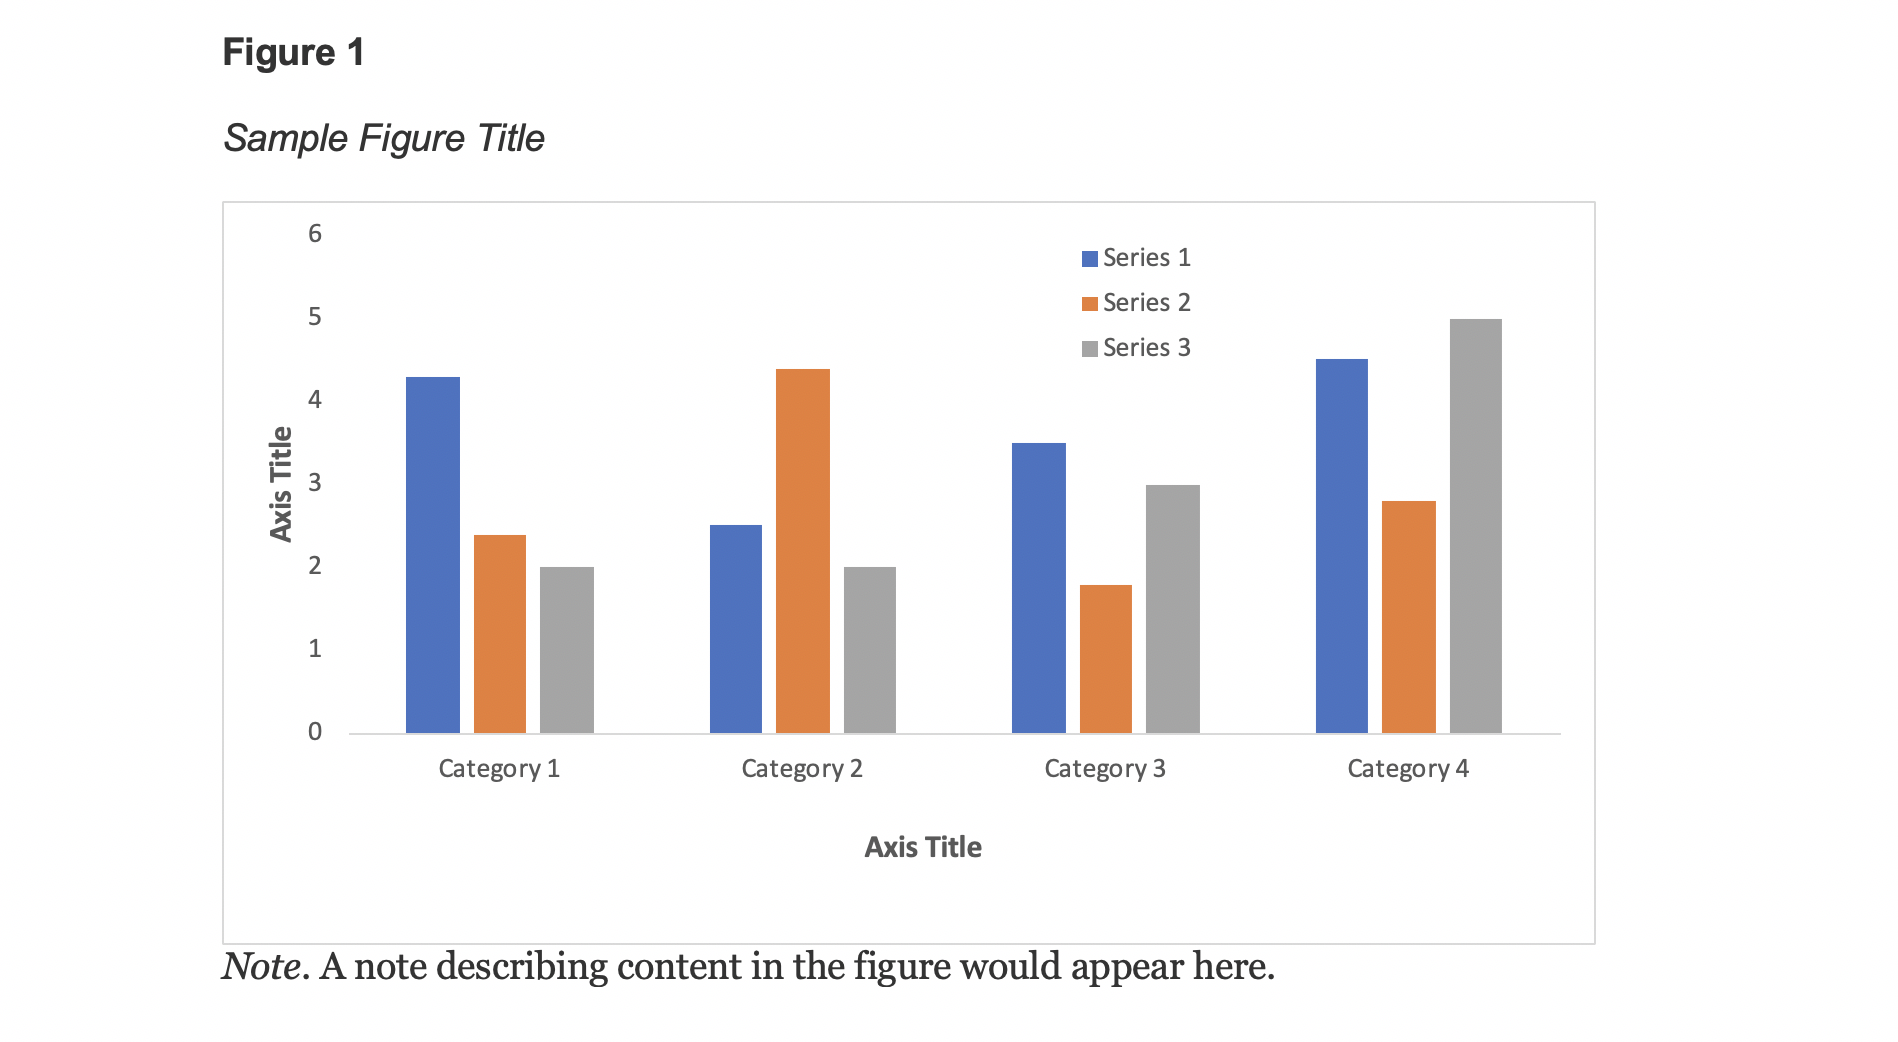
\includegraphics[width=1.0\textwidth]{figures/fig1.png}
    \caption{Sample figure showing a graph}
    \label{fig:sample_figure}
\end{figure}

This is sample algoritm. You can refer it as \ref{alg:bubblesort}.

\begin{algorithm}
\caption{Sample Algorithm: Bubble Sort}
\label{alg:bubblesort}
\KwIn{An array A of n elements}
\KwOut{Array A sorted in ascending order}
\Begin{
    \For{i = 0 to n - 1}{
        \For{j = 0 to n - i - 1}{
            \If{A[j] > A[j + 1]}{
                swap A[j] and A[j + 1]
            }
        }
    }
}
\end{algorithm}


This is a sample equation. You can refer it as \ref{eqn:quadratic}.

\begin{equation}
    \label{eqn:quadratic}
    x = \frac{-b \pm \sqrt{b^2 - 4ac}}{2a}
\end{equation}
\chapter{CONCLUSION AND FUTURE WORK}
\lipsum[15-20]

%do not remove this line
%This is the end of your text.
\makereferences

%keep here as it is.
\makeatletter
\ifx\@thesistype\@phdthesistype
    \makecv
\fi
\makeatother
%keep here as it is.
%if you have supplemantary data, uncomment the following line.
\iffilenotempty{supplementary.tex}{\makesupplementary}
% Your supplementary material goes here

\end{document}